\documentclass{article}
\usepackage{algpseudocode}
\usepackage{algorithm}
\usepackage{graphicx}
\usepackage{amsmath}
\DeclareMathOperator*{\argmax}{arg\,max}

\title{Report of hybrid algorithms}
\author{Yin Zhou}
\date{\today}

\begin{document}
	
	\maketitle
	
	\newpage
	
	\begin{algorithm}
		\caption{Combine Policy Gradient with Evolution Strategies (PGES)}
		\label{alg1}
		\textbf{Hyperparameters:
			\\ \hspace*{.5cm} learning rate: $\alpha$
			\\ \hspace*{.5cm} number of iteration: $num$
			\\ \hspace*{.5cm} population size: $pop$
			\\ \hspace*{.5cm} number of generation: $g$
			\\ \hspace*{.5cm} sigma: $\sigma$
			\\ \hspace*{.5cm} batch size: $n$
			\\	Axioms:
%			\\ \hspace*{.5cm} exponential weighted average improvement: $ave\_imp$
%			\\ \hspace*{.5cm} improvement: $imp$
			\\ \hspace*{.5cm} objective function: $J$
			\\ \hspace*{.5cm} network parameters: $\theta$}
		
%		\\hrulefill
		
		\begin{algorithmic}
			\\\hrulefill
			%\State $ i \gets 1 $
			%\Repeat 
			\State Initialize $\theta_{0}$ 
     		\State $last\_return = 0$
			\For{$iter \gets 1, ..., n$}
			\State Sampling trajectories 
			\State Estimate gradients $\nabla_{\theta} J$ 
			\State $\theta_{i+1} = \theta_{i} + \nabla_{\theta} J$
			%\While {$ i > 10 $}
			%\State statement
			\If{$current\_return \le last\_return * 0.9$}
			\State{Initialize $\{\epsilon_{j}\}_{j=1}^{pop}$}
			\State{then initialize population  $\{\theta_{j}\}_{j=1}^{pop}$ around $\theta_{i+1}$ and estimate the  \\ \hspace{0.95cm} expected returns of each individual $\{F_{j}\}_{j=1}^{pop}$}
			\State{$\theta = \theta + \alpha * \frac{1}{n\sigma} \Sigma_{j=1}^{pop} F_{j} \epsilon_{j}$}
			\For{$gen \gets 1, g$}
			\State Generate new population from the center 
			\State Repeat the update process for the center
			%\State statement
			\EndFor
			\State $last\_return = current\_return$
			\EndIf
			%\EndWhile
			\EndFor
			%\Until Finish all iterations
		\end{algorithmic}
	\end{algorithm}

\newpage
\section{Results for CartPole-v0}

\begin{figure}[htbp]
	\centering
	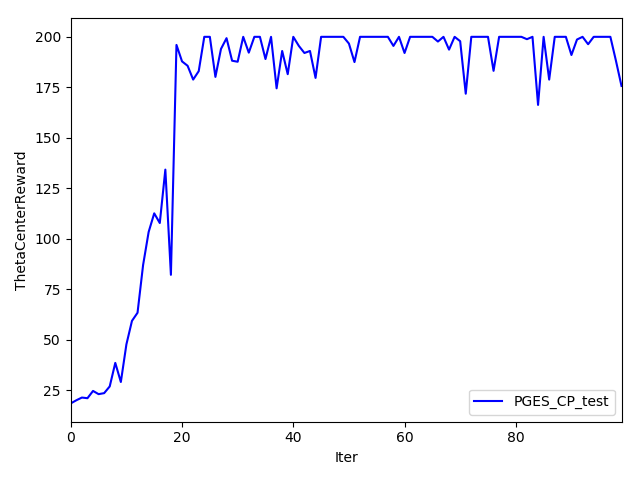
\includegraphics[width=1.00\textwidth]{PGES_CP_test.png}
	\caption{CartPole-v0}\label{fig:digit}
\end{figure}

\large{\noindent python PGES.py CartPole-v0 -n 100  -b 5000  -e 5  -rtg  -l 1  -s 32 \\ --exp name PGES\_CP\_test} \\
\large{Performance similar to Policy Gradient, but slower.}

\newpage
\section{Results for InvertedPendulum-v2}

\begin{figure}[htbp]
	\centering
	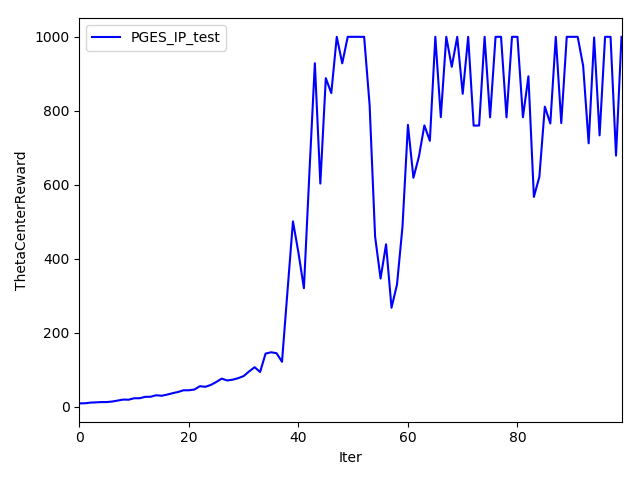
\includegraphics[width=1.00\textwidth]{PGES_IP_test.png}
	\caption{InvertedPendulum-v2}\label{fig:digit}
\end{figure}
\large{\noindent python PGES.py InvertedPendulum-v2 -n 100  -b 2000  -e 1  -rtg  -l 1  -s 32 -lr 0.005 -ts -tm --exp name PGES\_IP\_test} \\

\newpage
\section{Results for HalfCheetah-v2}

\begin{figure}[htbp]
	\centering
	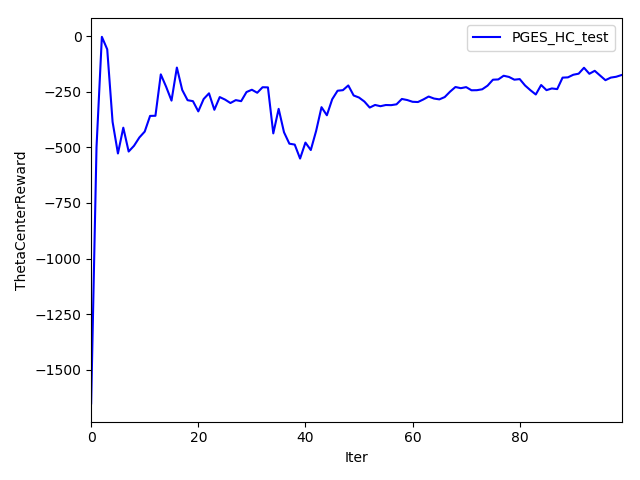
\includegraphics[width=1.00\textwidth]{PGES_HC_test.png}
	\caption{InvertedPendulum-v2}\label{fig:digit}
\end{figure}

\large{Results are really bad.}
	

\end{document}